\documentclass[conference,twocolumn]{IEEEtran}
\usepackage{blindtext}
\usepackage[utf8]{inputenc} 
\usepackage{cmap}
\usepackage[T1]{fontenc}

\usepackage[german]{babel}
\usepackage[babel,german=quotes]{csquotes}
%\selectlanguage{ngerman}
%\documentclass[conference]{../sty/IEEEtran}

%\usepackage{ifpdf}

%\ifpdf
%pdf code
%\else
%dvi code
%\fi

% \ifCLASSINFOpdf conditional that works the same way.

% *** CITATION PACKAGES ***
%
% \usepackage{cite}
% cite.sty was written by Donald Arseneau
% V1.6 and later of IEEEtran pre-defines the format of the cite.sty package
% \cite{} output to follow that of IEEE. Loading the cite package will
% result in citation numbers being automatically sorted and properly
% "compressed/ranged". e.g., [1], [9], [2], [7], [5], [6] without using
% cite.sty will become [1], [2], [5]--[7], [9] using cite.sty. cite.sty's
% \cite will automatically add leading space, if needed. Use cite.sty's
% noadjust option (cite.sty V3.8 and later) if you want to turn this off.
% cite.sty is already installed on most LaTeX systems. Be sure and use
% version 4.0 (2003-05-27) and later if using hyperref.sty. cite.sty does
% not currently provide for hyperlinked citations.
% The latest version can be obtained at:
% http://www.ctan.org/tex-archive/macros/latex/contrib/cite/
% The documentation is contained in the cite.sty file itself.

% *** GRAPHICS RELATED PACKAGES ***
%
%\ifCLASSINFOpdf
  \usepackage[pdftex]{graphicx}
  \graphicspath{{/img/}}
  \DeclareGraphicsExtensions{.pdf,.jpeg,.png}
%\else
%  \usepackage[dvips]{graphicx}
%  \graphicspath{{/img/}}
%  \DeclareGraphicsExtensions{.eps}
%\fi

% *** MATH PACKAGES ***
%
\usepackage[cmex10]{amsmath}

\interdisplaylinepenalty=2500

% *** SPECIALIZED LIST PACKAGES ***
%
%\usepackage{algorithmic}
% algorithmic.sty was written by Peter Williams and Rogerio Brito.
% This package provides an algorithmic environment fo describing algorithms.
% You can use the algorithmic environment in-text or within a figure
% environment to provide for a floating algorithm. Do NOT use the algorithm
% floating environment provided by algorithm.sty (by the same authors) or
% algorithm2e.sty (by Christophe Fiorio) as IEEE does not use dedicated
% algorithm float types and packages that provide these will not provide
% correct IEEE style captions. The latest version and documentation of
% algorithmic.sty can be obtained at:
% http://www.ctan.org/tex-archive/macros/latex/contrib/algorithms/
% There is also a support site at:
% http://algorithms.berlios.de/index.html
% Also of interest may be the (relatively newer and more customizable)
% algorithmicx.sty package by Szasz Janos:
% http://www.ctan.org/tex-archive/macros/latex/contrib/algorithmicx/


% *** ALIGNMENT PACKAGES ***
%
\usepackage{array}

\usepackage{mdwmath}
\usepackage{mdwtab}

\usepackage{eqparbox}
% Also of notable interest is Scott Pakin's eqparbox package for creating
% (automatically sized) equal width boxes - aka "natural width parboxes".
% Available at:
% http://www.ctan.org/tex-archive/macros/latex/contrib/eqparbox/





% *** SUBFIGURE PACKAGES ***
%\usepackage[tight,footnotesize]{subfigure}
% subfigure.sty was written by Steven Douglas Cochran. This package makes it
% easy to put subfigures in your figures. e.g., "Figure 1a and 1b". For IEEE
% work, it is a good idea to load it with the tight package option to reduce
% the amount of white space around the subfigures. subfigure.sty is already
% installed on most LaTeX systems. The latest version and documentation can
% be obtained at:
% http://www.ctan.org/tex-archive/obsolete/macros/latex/contrib/subfigure/
% subfigure.sty has been superceeded by subfig.sty.


%\usepackage[caption=false]{caption}
%\usepackage[font=footnotesize]{subfig}
% subfig.sty, also written by Steven Douglas Cochran, is the modern
% replacement for subfigure.sty. However, subfig.sty requires and
% automatically loads Axel Sommerfeldt's caption.sty which will override
% IEEEtran.cls handling of captions and this will result in nonIEEE style
% figure/table captions. To prevent this problem, be sure and preload
% caption.sty with its "caption=false" package option. This is will preserve
% IEEEtran.cls handing of captions. Version 1.3 (2005/06/28) and later 
% (recommended due to many improvements over 1.2) of subfig.sty supports
% the caption=false option directly:
%\usepackage[caption=false,font=footnotesize]{subfig}
%
% The latest version and documentation can be obtained at:
% http://www.ctan.org/tex-archive/macros/latex/contrib/subfig/
% The latest version and documentation of caption.sty can be obtained at:
% http://www.ctan.org/tex-archive/macros/latex/contrib/caption/


% *** FLOAT PACKAGES ***
%
%\usepackage{fixltx2e}
% fixltx2e, the successor to the earlier fix2col.sty, was written by
% Frank Mittelbach and David Carlisle. This package corrects a few problems
% in the LaTeX2e kernel, the most notable of which is that in current
% LaTeX2e releases, the ordering of single and double column floats is not
% guaranteed to be preserved. Thus, an unpatched LaTeX2e can allow a
% single column figure to be placed prior to an earlier double column
% figure. The latest version and documentation can be found at:
% http://www.ctan.org/tex-archive/macros/latex/base/

%\usepackage{stfloats}
% stfloats.sty was written by Sigitas Tolusis. This package gives LaTeX2e
% the ability to do double column floats at the bottom of the page as well
% as the top. (e.g., "\begin{figure*}[!b]" is not normally possible in
% LaTeX2e). It also provides a command:
%\fnbelowfloat
% to enable the placement of footnotes below bottom floats (the standard
% LaTeX2e kernel puts them above bottom floats). This is an invasive package
% which rewrites many portions of the LaTeX2e float routines. It may not work
% with other packages that modify the LaTeX2e float routines. The latest
% version and documentation can be obtained at:
% http://www.ctan.org/tex-archive/macros/latex/contrib/sttools/
% Documentation is contained in the stfloats.sty comments as well as in the
% presfull.pdf file. Do not use the stfloats baselinefloat ability as IEEE
% does not allow \baselineskip to stretch. Authors submitting work to the
% IEEE should note that IEEE rarely uses double column equations and
% that authors should try to avoid such use. Do not be tempted to use the
% cuted.sty or midfloat.sty packages (also by Sigitas Tolusis) as IEEE does
% not format its papers in such ways.


% *** PDF, URL AND HYPERLINK PACKAGES ***
%
\usepackage{url}
% url.sty was written by Donald Arseneau. It provides better support for
% handling and breaking URLs. url.sty is already installed on most LaTeX
% systems. The latest version can be obtained at:
% http://www.ctan.org/tex-archive/macros/latex/contrib/misc/
% Read the url.sty source comments for usage information. Basically,
% \url{my_url_here}.

% correct bad hyphenation here
\hyphenation{op-tical net-works semi-conduc-tor}

% Bib
%\bibliographystyle{IEEEtran}

\usepackage[%
 backend=biber,%
 style=numeric,%
% bibstyle=alphabetic,%
% citestyle=alphabetic,%
 natbib=true,%
 sorting=anyt,%
 sortcites=true,%
 hyperref=auto,%
 maxnames=3,%
 minnames=1,%
]{biblatex}

\bibliography{bibo.bib}

\begin{document}

\title{Ansätze zur Parameteridentifikation der PMSM}

\author{\IEEEauthorblockN{Benjamin Ternes, IEEE Member}
\IEEEauthorblockA{Hochschule Bochum\\
Fachbereich Elektrotechnik und Informatik\\
Bochum, Germany\\
E-mail: benjamin.ternes@hs-bochum.de\\
GitHub: \url{https://github.com/benjiternes/}}
\and
\IEEEauthorblockN{Jan Feldkamp}
\IEEEauthorblockA{Hochschule Bochum\\
Fachbereich Elektrotechnik und Informatik\\
Bochum, Germany\\
E-mail: jan.feldkamp@hs-bochum.de}}
%\and
%\IEEEauthorblockN{James Kirk\\ and Montgomery Scott}
%\IEEEauthorblockA{Starfleet Academy\\
%San Francisco, California 96678-2391\\
%Telephone: (800) 555--1212\\
%Fax: (888) 555--1212}}

% conference papers do not typically use \thanks and this command
% is locked out in conference mode. If really needed, such as for
% the acknowledgment of grants, issue a \IEEEoverridecommandlockouts
% after \documentclass

% for over three affiliations, or if they all won't fit within the width
% of the page, use this alternative format:
% 
%\author{\IEEEauthorblockN{Michael Shell\IEEEauthorrefmark{1},
%Homer Simpson\IEEEauthorrefmark{2},
%James Kirk\IEEEauthorrefmark{3}, 
%Montgomery Scott\IEEEauthorrefmark{3} and
%Eldon Tyrell\IEEEauthorrefmark{4}}
%\IEEEauthorblockA{\IEEEauthorrefmark{1}School of Electrical and Computer Engineering\\
%Georgia Institute of Technology,
%Atlanta, Georgia 30332--0250\\ Email: see http://www.michaelshell.org/contact.html}
%\IEEEauthorblockA{\IEEEauthorrefmark{2}Twentieth Century Fox, Springfield, USA\\
%Email: homer@thesimpsons.com}
%\IEEEauthorblockA{\IEEEauthorrefmark{3}Starfleet Academy, San Francisco, California 96678-2391\\
%Telephone: (800) 555--1212, Fax: (888) 555--1212}
%\IEEEauthorblockA{\IEEEauthorrefmark{4}Tyrell Inc., 123 Replicant Street, Los Angeles, California 90210--4321}}

% use for special paper notices
%\IEEEspecialpapernotice{(Invited Paper)}

\maketitle

\begin{abstract}
\boldmath
Synchronmaschinen mit Permanentmagneterregung werden in vielen Anwendungen eingesetzt.
Oftmals sind dies Anwendungen, die eine hochdynamische Regelung erfordern.
Aus Kosten- und Wartungsgründen wird oft auf einen Drehgeber verzichtet, die Lage wird dann \enquote{geberlos} aus den Kenngrößen geschätzt.
Die hochdynamischen \enquote{geberlosen} Regelungen benötigen die Induktivitäten der Maschine nicht nur als konstante Größen, sondern abhängig von den momentanen Strömen \autocite{Kellner2012}.
Die Flussverkettung der Permanentmagnete ändert sich aufgrund von Alterungserscheinungen und Temperaturveränderungen im Laufe des Betriebs.
Der ohmsche Ständerwiderstand, der sich durch Erwärmung des Ständers im Laufe des Betriebs verdoppeln kann, wird zur Drehmomentsberechnung benötigt.
Induktivitäten können auf verschiedene Arten gemessen werden.
Im Rahmen der Maschinenauslegung durchgeführten Finite-Elemente-Methode und Berechnung der Induktivitäten auf dieser Basis.
Auf der Basis berechnete Induktivitäten entstanden im Zusammenhang mit einem vereinfachten Modell, das dennoch realistische Werte liefern soll.
Bei realen Maschinen können in der Fertigungstoleranzen auftreten und zum anderen werden die Wickelköpfe der Maschinen in der FEM-Berechnung nicht berücksichtigt.
Aus diesen Gründen ist es sinnvoll, die Induktivitäten an der realen Maschine zu messen.
Dazu werden im Folgenden zwei Ansätze zur Berechnung dargestellt: Injektion von Testsignalen im Stillstand der Maschine, die sog. differentiellen Induktivitäten zu bestimmen und bei konstanter Drehzahl die absoluten Induktivitäten zu identifizieren.
Sind diese Induktivitäten gemessen, so können sie gespeichert und für die hochdynamische Regelung verwendet werden.
Den ohmschen Ständerwiderstand der Synchronmaschine muss man während des Betriebes identifizieren.
\end{abstract}

\begin{IEEEkeywords}
PMSM, Identifikation, Induktivitäten
\end{IEEEkeywords}


% For peer review papers, you can put extra information on the cover
% page as needed:
% \ifCLASSOPTIONpeerreview
% \begin{center} \bfseries EDICS Category: 3-BBND \end{center}
% \fi
%
% For peerreview papers, this IEEEtran command inserts a page break and
% creates the second title. It will be ignored for other modes.
\IEEEpeerreviewmaketitle

\tableofcontents

\section{Mathematisches Modell der PMSM}\label{sec:math-pmsm}

Grundlegende Beschreibungen elektrischer Maschinen liefern Standardwerke, wie z.~B.\ \autocites{mullerII2008}{mullerI2005}{fischer2009}{schroder2000}.
In der vorliegenden Arbeit sind die in der Regel verwendeten linearisierten Spannungsgleichungen mit konstanten elektrischen Parametern allerdings nicht mehr ausreichend.
In dieser Arbeit werden Ansätze zur Erweiterung der linearisierten Gleichungen dargestellt.
Einige Ansätze unterteilen die absoluten Induktivitäten $L_d$ und $L_q$ in zwei Selbst- und Gegeninduktivitäten.
Bei \autocite{sturmberger} sind dabei sowohl die Selbst- als auch die Gegeninduktivität jeweils von de Strömen $i_d$ und $i_q$ abhängig.
In dieser Arbeit wird eine absolute Induktivität in $d-$ und $q-$Richtung verwendet.
Dies hat den Vorteil, dass bei Vereinfachungen wieder ein lineares Gleichungssystem entsteht.
Dabei werden allerdings die Eisenverluste nicht berücksichtigt.
Diese sind aber notwendig, um Induktivitäten zu messen und insbesondere den ohmschen Ständerwiderstand zu identifizieren \autocite{Kellner2012}.
Alle folgenden Anpassungen des Maschinenmodells beziehen sich weiterhin nur auf das Grundwellenverhalten der Maschine.
Eine Zusätzliche Betrachtung der Oberwelleneffekte wird innerhalb dieser Arbeit nicht weiter betrachtet.

Reduziert man die Synchronmaschine auf ihre grundlegenden elektrischen Eigenschaften so ergibt sich nach Abb.~\ref{fig:synchron-grundlage}: Drei Induktivitäten im Ständerblechpacket zusammen mit dem Permanentmagneten im Läufer.

\begin{figure}
\centering
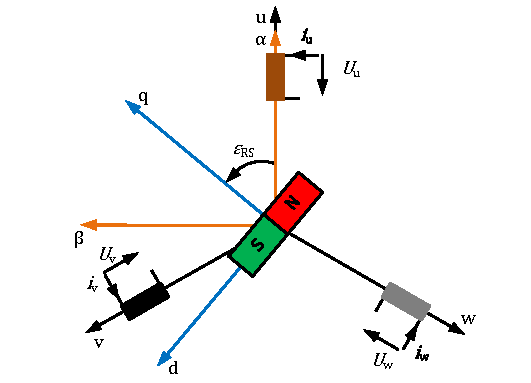
\includegraphics[width=\columnwidth]{img/synchron-grundlage}
\label{fig:synchron-grundlage}
\caption{Graphische Veranschaulichung der verschiedenen Koordinatensysteme, ständerfest $(\alpha, \beta)$ und rotorfest $(d, q)$.}
\end{figure}

Nach \textcite{ternesfeldkamp} und Transformation in das ständerfeste $(\alpha, \beta)$-Koordinatensystem ergibt sich die Spannungsleichung im rotorfesten System zu

\begin{align}
u_d &= R_1 i_d + \frac{d}{dt}\Psi_d - \omega_{el} \Psi_q \label{eqn:ud} \\ 
u_q &= R_1 i_q + \frac{d}{dt}\Psi_q + \omega_{el} \Psi_d \label{eqn:uq}
\end{align}

Allgemein lässt sich das daraus resultierende innere Drehmoment als

\begin{align}
M_i = \frac{3}{2} \underline{\Psi}^{d,q} \times \underline{i}^{d,q} \label{drehmoment}
\end{align}

beschreiben.
Dabei wird vorausgesetzt, dass die Ständerwicklung symmetrisch und dreiphasig ist, der Strombelag nach \textcite{ternesfeldkamp} sinusförmig über dem Umfang verteilt und kein Nullsystem vorliegt.
Das innere Drehmoment $M_i$ für eine Maschine mit $p$ Polpaaren kann nach der Berechnung des Vektorproduktes als

\begin{align}
M_i = \frac{3p}{2}(\Psi_d i_q - \Psi_q i_d)
\end{align}

definiert werden.
Um das System vollständig zu beschreiben fehlt noch die Bewegungsgleichung nach \textcite{mullerI2005}.

\begin{align}
M_i - M_L = J \frac{d}{dt} \omega_{mech} \label{bewegungsgleichung}
\end{align}

Bei diesem Modell sind alle Parameter konstant, die Ableitungen der Flussverkettungen, die in Gl.~(\ref{eqn:ud}) und Gl.~(\ref{eqn:uq}) verwendet werden unkompliziert zu bestimmen.
Aufgrund von Sättigungseffekten des Eisens sind insbesondere bei hochausgenutzten Maschinen die Induktivitäten der Synchronmaschine nicht mehr konstant, sondern vom Motorstrom abhängig \autocite{Kellner2012}.

\subsection{Linearisierte Gleichungen}\label{sec:lin-gleichungen}

Bei dem linearisierten Modell sind definitionsgemäß \autocite{mullerII2008} keine Sättigungserscheinungen vorhanden.
Alle elektrischen Parameter der Permanentmagneterregten Synchronmaschine und damit auch die Induktivitäten sind damit konstant.
Aus dieser Annahme folgt nach \textcite{ternesfeldkamp}, dass sich in läuferfesten $d, q-$Komponenten

\begin{align}
\Psi_d &= \Psi_pm + L_d i_d \\
\Psi_q &= L_q i_q
\end{align}

ergeben.
Die in $d-$Achse ausgerichteten Permanentmagnete rufen eine als konstant angenommene Flussverkettung $\Psi_pm$ hervor.
Daraus ergeben sich in Gl.~(\ref{eqn:ud}), Gl.~(\ref{eqn:uq}) und Gl.~(\ref{drehmoment}) eingesetzt~--~die Grundgleichungen des linearen Maschinenmodells

\begin{align}
u_d &= R_1 i_d + L_d \frac{di_d}{dt} - \omega_{el}L_q i_q  \label{uq-allg} \\ 
u_q &= R_1 i_q + L_q \frac{di_q}{dt} + \omega_{el}L_d i_d + \omega_{el}\Psi_pm \label{ud-allg} \\ 
M_i &= \frac{3p}{2}(\Psi_pm i_q + (L_d - L_q)i_d i_q)
\end{align}

Die Spannungsgleichungen lassen sich gemäß Abb.~\ref{fig:spannungsgleichungen} graphisch darstellen.

\begin{figure}
%\centering
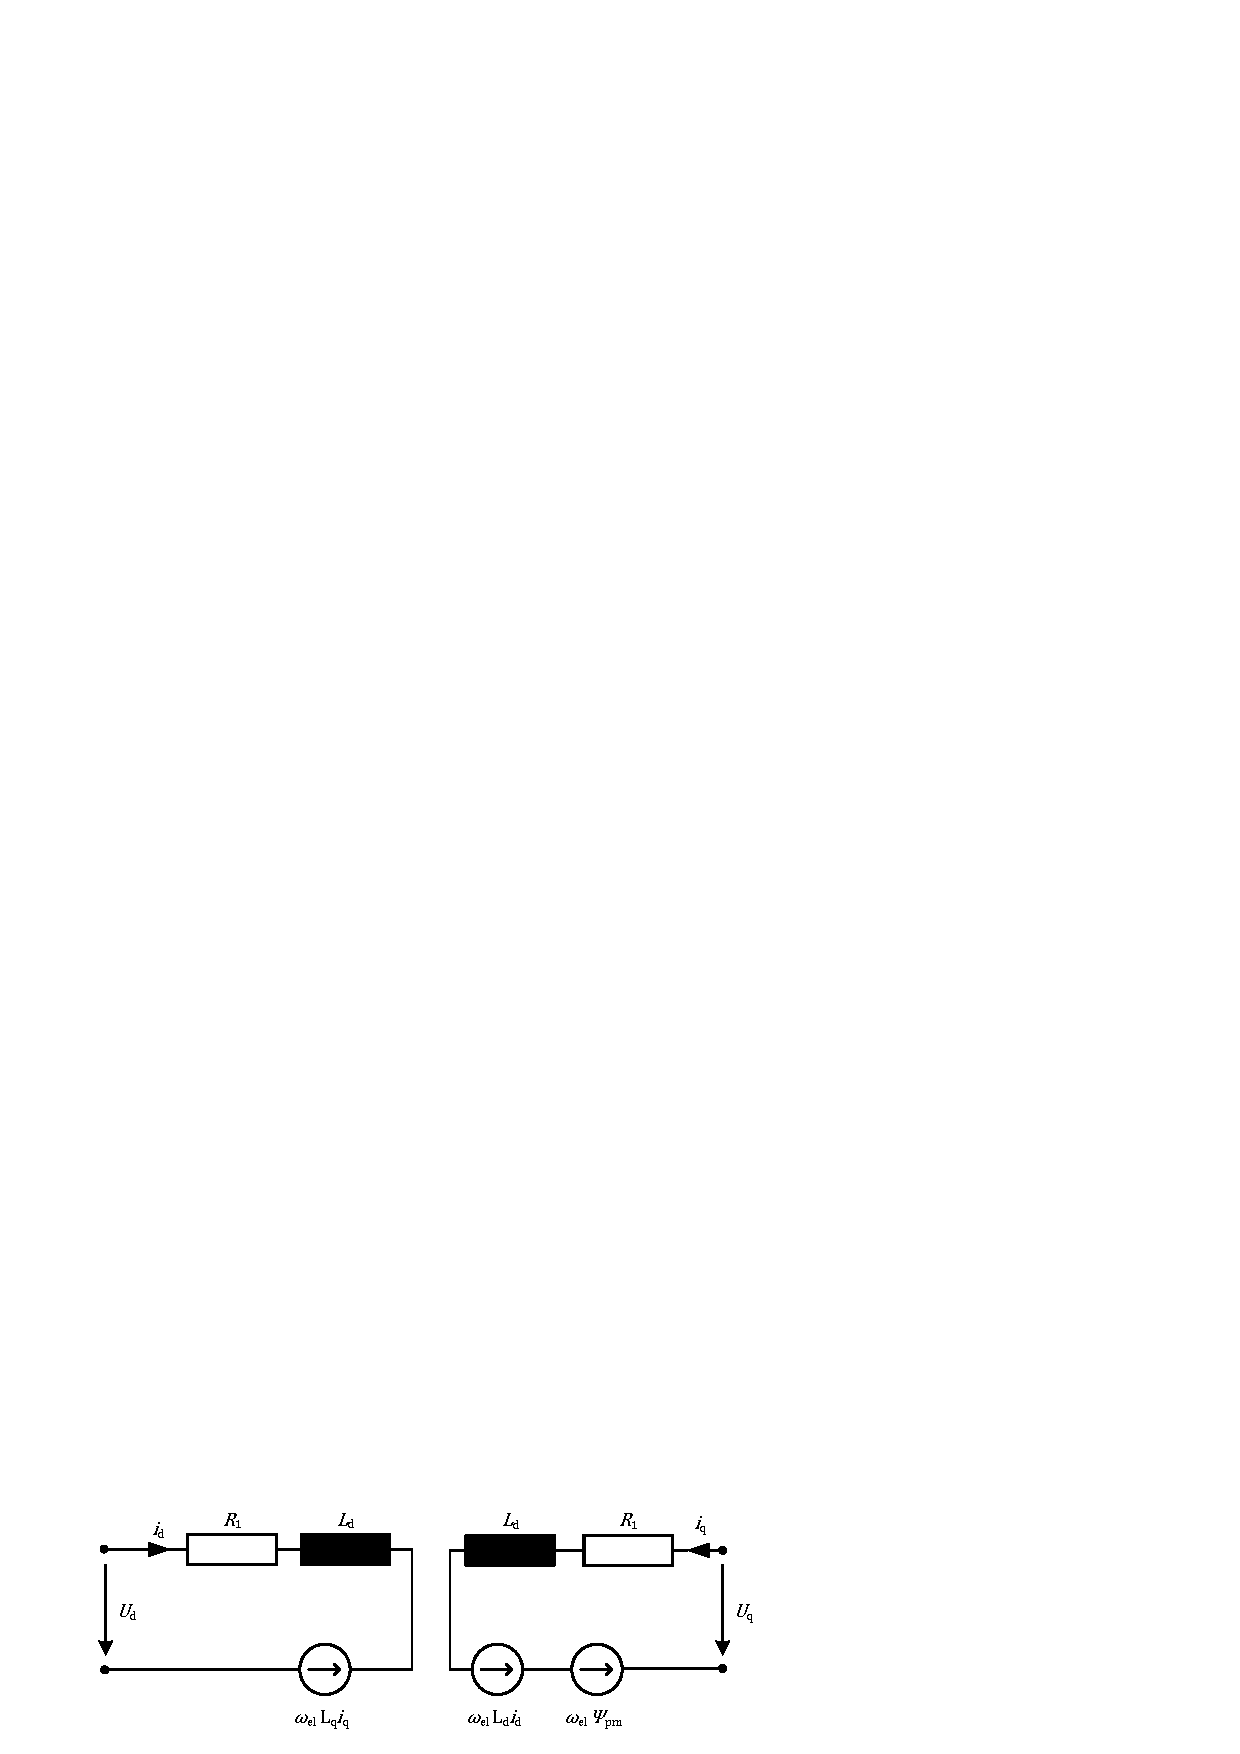
\includegraphics[width=\columnwidth]{img/spannungsgleichungen}
\label{fig:spannungsgleichungen}
\caption{Graphische Darstellung der Gleichungen (\ref{ud-allg}) und (\ref{uq-allg}).}
\end{figure}

Erkennbar ist, dass in der Abb.~\ref{fig:spannungsgleichungen} die Spannungsquellen $\omega_el L_q i_q$ und $\omega_el L_d i_d$ miteinander verkoppelt sind.
Löst man oben stehende Gl.~(\ref{uq-allg},\ref{ud-allg}) mit der Bewegungsgleichung Gl.~(\ref{bewegungsgleichung}), so erhält man in Zustandsform

\begin{align}
\frac{di_d}{dt} &= -\frac{R_1}{L_d}i_d+\omega_{el}\frac{L_q}{L_d}i_q+\frac{1}{L_d}u_d \\
\frac{di_q}{dt} &= -\omega_{el}\frac{L_d}{L_q}i_d - \frac{R_1}{L_q}i_q + \frac{1}{L_q}u_q-\frac{\omega_{el}}{L_q}\Psi_{pm} \\
\frac{d\omega_{el}}{dt} &= \frac{3p^2}{2J}(L_d - L_q)i_q i_d + \frac{3p^2}{2J} \Psi_{pm} i_q - \frac{p}{J} M_L
\end{align}

\section{Ansätze zur Identifikation}\label{sec:identifikation}

Um die Parameter einer PMSM identifizieren zu können, ist es notwendig die korrekte Lage des Rotors festzustellen \autocites{underwood_online_2010}{rahman_identification_2005}{piippo_adaptation_2009}.
Mit Hilfe eines Resolvers, Inkrementalgeber oder einen Absolutwertgeber wird die Rotorlage ermittelt.
Die Implementierung solcher Messeinrichtungen ist mit Kosten und Wartungsaufwand verbunden und nicht immer nachrüstbar.
An dieser Stelle soll deshalb auf eine geberlose Regelung eingegangen werden.
Wie die Bezeichnung schon nahelegt, wird bei der geberlosen Regelung auf den Drehgeber verzichtet.
Bei einer geberlosen Regelung werden i.\ d.\ R.\ aus den drei Phasenströmen der Läuferlagewinkel berechnet, wobei von den drei Phasenströmen nur zwei gemessen werden und der dritte wird aus ihnen berechnet \autocite{slotine_applied_1991}.
Es gibt unzählige Veröffentlichungen in diesem Forschungsbereich, dabei werden auch unterschiedliche Verfahren zur Realisierung dargestellt.
Im folgenden soll aber auf eine Unterscheidung und den Vergleich unterschiedlicher Implementierungsvarianten nicht eingegangen werden.

%\emph{Testsignale für niedrige Drehzahlen:}

\emph{EMK-Verfahren für hohe Drehzahlen:} Im Gegensatz zu dem beschriebenen Testsignalverfahren, welches aktiv in das Antriebssystem eingreift, ergeben sich bei hohen Drehzahlen genügend passive Verfahren zur Bestimmung der Rotorlage.

\begin{quote}
\enquote{[\ldots] Eine Drehzahl ist immer dann für das EMK-Verfahren ausreichend, wenn die angelegten Spannungen so groß sind, dass der Rauschanteil auf den gemessenen oder berechneten Spannungen vernachlässigbar klein ist. [\ldots] \autocite[S.~48]{Kellner2012}}
\end{quote}

Basis für solche EMK-Modelle sind die in Abschn.~\ref{sec:lin-gleichungen} beschriebenen Gleichungen.
Dabei wird von einem linearen Verhalten im Betriebsbereich ausgegangen \autocite{piippo_adaptation_2009}.

\subsection{Berücksichtigung der Eisenverluste}\label{sec:eisenverluste}

Bisher wurden in den beschriebene Gleichungen nur die ohmschen Verluste betrachtet.
Seit Anfang des 20. Jahrhunderts ist jedoch bekannt, dass neben den ohmschen Verlusten im Kupfer des Ständers weitere Verluste in den elektrischen Maschinen auftreten \autocites{reinert_calculation_2001}{stumberger_evaluation_2003}{kilthau_parameter-measurement_2001}{sturmberger}.
Diese Verluste werden als \enquote{Eisenverluste} zusammengefasst und beinhalten Wirbelstromverluste durch Läufer- und Ständerblechpacket.
Außerdem treten auch Hystereseverluste auf, die durch die Ummagnetisierung des Eisenblechs bedingt sind.
Hier wird auf weiterführende Literatur empfohlen, s.~h. \textcites{reinert_calculation_2001}{stumberger_evaluation_2003}{kilthau_parameter-measurement_2001}{sturmberger}.
Eine gesonderte Untersuchung dieser beiden Effekte ist allerdings nicht sinnvoll, da Wirbelstrom- und Hystereseverluste den gleichen physikalischen Effekt beschreiben \autocite{reinert_calculation_2001}.
Eine getrennte Messung ist in der Praxis schwer zu realisieren.
Zu den Eisenverlusten kommen noch einige parasitäre Effekte, wie Ständerverluste, durch eine nichtsinusförmige Speisung der Motoren, insb. durch Pulsumrichter \autocite{Kellner2012}.
Auf dem Forschungsgebiet besteht noch große Uneinigkeit, so schreibt \textcite{Kellner2012} in seiner Dissertation

\begin{quote}
\enquote{[\ldots] Es ist zu erkennen, dass auf dem Forschungsgebiet der analytischen Beschreibung
der Eisenverluste große Uneinigkeit über deren Art und Weise besteht. [\ldots] Daher ist bislang
noch kein allgemeingültiger Lösungsansatz zur analytischen Beschreibung der
Eisenverluste gelungen. \autocite[S.~65]{Kellner2012}} 
\end{quote}

Für die Identifikation der Eisenverluste bietet es sich an, die Maschine mit einem Teststrom zu speisen.
Dafür muss zwingend eine Vorschrift für die Beschreibung der Eisenverluste eingeführt werden, s.~h. \autocite[S.~75]{Kellner2012}.

\subsection{Identifikation des Stränderwiderstands}\label{sec:sident}

Der Ständerwiderstand $R_1$ ist eine wichtige Kenngröße für den Betrieb elektrischer Maschinen.
Bei dem modellbasierten EMK-Verfahren für kleine Drehzahlen, z. B. \autocite{genduso}, ist es notwendig eine möglichst genauen Ständerwiderstand zu bekommen.
Im folgenden werde einige Beispiele zur Identifikation des Ständerwiderstandes anhand aktueller Literatur dargestellt.

Die Auswertung der $u_d-$ oder $u_q-$Spannungsgleichung: Zur Auswertung der $u_d$-Gleichung ist ein $d-$Strom ungleich null Voraussetzung, was die praktische Anwendung stark einschränkt \autocite{Kellner2012}.
Die Auswertung der $u_q-$Gleichung liefert immer dann gute Ergebnisse, wenn gleichzeitig hohe $i_d-$Ströme und kleine Drehzahlen vorhanden sind.
Für die Antriebe die aus dem Stand anfahren, ist dies kein Nachteil.
Es gibt auf dem Gebiet \enquote{Verfahren zur Identifikation der Parameter von permanenterregten Synchronmaschinen} viele Veröffentlichungen.
Viele Autoren verwenden den \texttt{MRAC}-Algorithmus (model-reference adaptive control) zur Identifikation des Ständerwiderstandes \autocite{slotine_applied_1991}.
Der prinzipielle Aufbau ist in Abb.~\ref{fig:synchron-grundlage} gezeigt.

\begin{figure}
%\centering
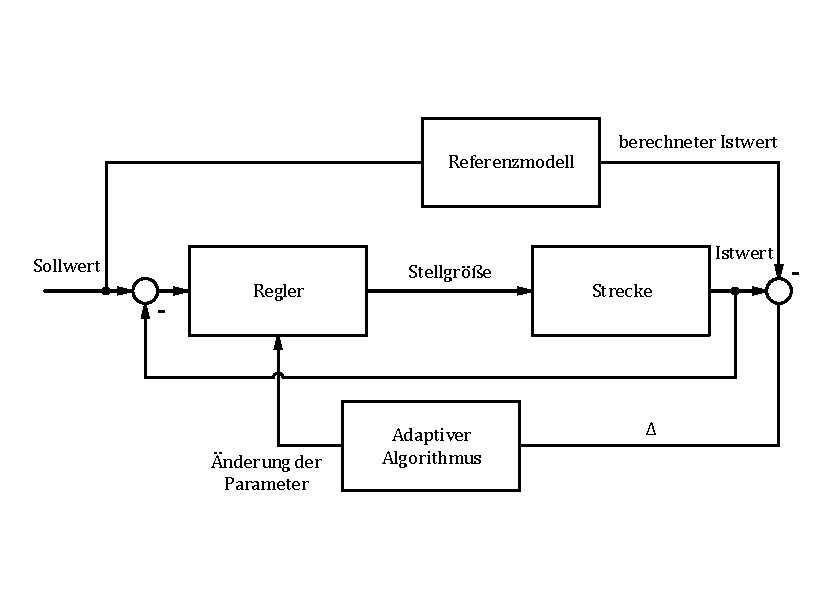
\includegraphics[width=\columnwidth]{img/mrac}
\label{fig:mrac}
\caption{Prinzipielle Darstellung eines \texttt{MRAC}-Algorithmus nach \textcite{slotine_applied_1991}.}
\end{figure}

Wenn bekannt ist, welchen Verlauf die Ausgangsgröße der Strecke bei einer bestimmten Eingangsgröße haben soll, dann kann diese mathematische Beziehung in einem Referenzmodell hinterlegt werden.
Der Algorithmus ist in \autocite{slotine_applied_1991} genauer beschrieben (s.~h.~Abb.~\ref{fig:mrac}).
Bei der Parameteridentifikation kann das mathematische Referenzmodell die Gleichungen der PMSM beschreiben, der Regler passt über den Ständerwiderstand die unbekannte Strecke an, bis sie den idealen Maschinengleichungen entsprechen.
Sind die Parameter der Maschine nicht genau bekannt, dann ist es nicht möglich ein genaues Referenzmodell zu erstellen.
Eine andere Möglichkeit zur Identifikation des Ständerwiderstandes ist die Einprägung von Testsignalen in $d-$ und $q-$Richtung.
Die Auswertung der eingeprägten Signale liefert dann die Spannungs- bzw. Stromantwort.
In: Wilson, S. D.; Jewell, G. W.; Stewart, P. G.: \emph{Resistance estimation for temperature determination in PMSMs through signal injection}. In: \emph{International Conferece on Eletric Maschines and Drives},(IEMDC)~--~(2005), pp. 735--740, wird eine Methode beschrieben, mit der durch Injektion eines Stromraumzeigers der Widerstand und damit auch die Temperatur der Ständerwicklung bestimmt wird.
Das Verfahren zur Bestimmung dieser Maschinen Parameter wurde bisher nur simuliert und nicht verifiziert.
Der entscheidende Nachteil dieses Prinzips ist, dass auch die Ständeridentifikation nur funktioniert, wenn das hochfrequente Testsignal vorhanden ist, also nur bei geringen Drehzahlen.
Weitere patentierte Identifikationsverfahren auf dem Gebiet sind in: Schutzrecht US 2008/0018288A1~--~\emph{Method of adjusting parameters
of a synchronous motor and variable speed drive using such a method} und Schutzrecht EP 1755211B1~--~\emph{Widerstandsschätzung eines elektrischen
Wechselstrommotors} beschrieben.
Weitere Ansätze zur Identifikation des Ständerwiderstandes sind in \textcite{Kellner2012} beschrieben, diese Verfahren benötigen keine Testsignale und werten die bekannten Spannungsgleichungen in $d-$ oder in $q-$Richtung in rotorfesten Koordinaten aus.
Diese Möglichkeit gilt nicht für alle Betriebsbereiche. 
Aus diesem Grund wird ein weiteres Verfahren eingeführt, welches robust und resourcenschonend ist.
Durch die Injektion eines niederfrequenten $i_d$-Strom-Testsignales kann die $u_d$-Spannungsgleichung ausgewertet werden.

\begin{figure}
%\centering
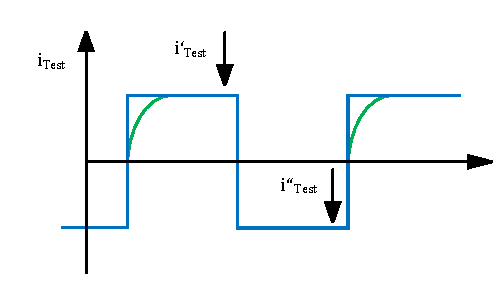
\includegraphics[width=\columnwidth]{img/test-strom}
\label{fig:test-strom}
\caption{Prinzipieller Teststromverlauf, Blau: Idealer Stromverlauf. Grün: Realer Stromverlauf.}
\end{figure}

Der gesamte Identifikationsprozess läuft innerhalb des rotorfesten $d, q-$Koordinatensystems ab.
Prinzipiell können sowohl die $u_d$-Spannungsgleichung, als auch die $u_q$-Spannungsgleichung verwendet werden.

\begin{quote}
\enquote{Die $u_q-$Gleichung scheidet jedoch aus: Der benötigte alternierende $i_q$-Teststrom würde ein unerwünschtes Pendelmoment erzeugen.}\autocite[S.~148]{Kellner2012}
\end{quote}

Der Einfluss in $d-$Richtung auf das abgegebene Drehmoment ist wesentlich geringer.
Damit kann die Gleichung für den identifizierten Ständerwiderstand nach \textcite{Kellner2012} geschrieben werden

\begin{align}
R_{1,ident} = \frac{1}{i_d''-i_d'} \cdot \left( u_d'' - u_d' + \omega_{el}'' L_q^{i_d'',i_q''}i_q'' - \omega'_{el}L_q^{i_d',i_q'}i_q' \right)
\end{align}

\subsection{Identifikation der Flussverkettung}\label{sec:ident-fluss}

Für die Identifikation der Flussverkettung $\Psi_{pm}$ kann das gleiche Testsignale in $d-$Richtung verwendet werden, wie bei der Identifikation des Ständerwiderstandes.
Bei der Identifikation des Flusses werden nur stationäre Zustände betrachtet \autocite{Kellner2012}, daher können die Ableitungen der Ströme weggelassen werden, da sie im Mittel ohnehin null ergeben.
Für die Identifikation des Flusses wird die $u_q-$Gleichung (s.~h.~Gl.~\ref{uq-allg}) verwendet.
Da der Teststrom nur in $d-$Richtung eingeprägt wird, kann $i_q$ als konstant angenommen werden.
Das Gleiche gilt für $\psi_{pm}$.
Durch Umformungen und vereinfachen der allgemeinen Gleichungen und der Annahme, dass $\omega_{el}=\textbf{const.}$ gilt nach \textcite{Kellner2012} für die Identifikation von $\Psi_{pm}$

\begin{align}
\tilde{\Psi}_{pm} = \frac{1}{2\tilde{\omega}_{el}} \left[ (u_q' + u_q'') - R_{1,ident}(i_q' + i_q'')- \tilde{\omega}_{el}\tilde{L}_d(i_d' + i_d'') \right]
\end{align}

mit $\tilde{\omega}_{el}=\frac{\omega_{el}'+\omega_{el}''}{2}$ und $\tilde{L}_d = \frac{1}{\tilde{\omega_{el}}}\cdot \frac{u_q'' - u_q'}{i_d''-i_d'}$

Das Verfahren entspricht der Mittelwertbildung aus den alternierenden Betriebszuständen, die durch die Testsignalspeisung für die Ständerwiderstandsidentifikation entstehen.
Andere Ansätze zur Identifikation des Flusses sind Theorien zur Geschwindigkeitsänderung und damit auch der Zustandsänderung.

\section{Parameterfehler}\label{sec:parameterfehler}

Zur Regelung von hochdynamischen elektrischen Maschinen, aber auch für deren Simulation sollten die Parameter der Maschine idealerweise exakt bekannt sein.
Je größer der Fehler ist, desto weniger bilden die Modelle die Realität ab.
Damit wird die Regeldynamik direkt verringert.
Ziel muss es also sein, die elektrischen Parameter~--~bei einer PMSM im wesentlichen der ohmsche Ständerwiderstand, der Permanentfluss und die Induktivitäten~--~möglichst exakt messbar sein.

Die Parameter $R_{1}, L$ und $Psi_{pm}$ können nicht direkt gemessen werden, sondern werden aus anderen gemessenen Größen berechnet.
Die resultierenden Probleme wirken sich auf die Drehmomentenberechnung und die Lagewinkelberechnung bei geberloser Regelung aus.
Beispiele für Fehler der Messgrößen sind Ungenauigkeiten der Umrichterlinearisierung oder Toleranzen der Stromsensoren.

% needed in second column of first page if using \IEEEpubid
%\IEEEpubidadjcol

% An example of a floating figure using the graphicx package.
% Note that \label must occur AFTER (or within) \caption.
% For figures, \caption should occur after the \includegraphics.
% Note that IEEEtran v1.7 and later has special internal code that
% is designed to preserve the operation of \label within \caption
% even when the captionsoff option is in effect. However, because
% of issues like this, it may be the safest practice to put all your
% \label just after \caption rather than within \caption{}.
%
% Reminder: the "draftcls" or "draftclsnofoot", not "draft", class
% option should be used if it is desired that the figures are to be
% displayed while in draft mode.
%
%\begin{figure}[!t]
%\centering
%\includegraphics[width=2.5in]{myfigure}
% where an .eps filename suffix will be assumed under latex, 
% and a .pdf suffix will be assumed for pdflatex; or what has been declared
% via \DeclareGraphicsExtensions.
%\caption{Simulation Results}
%\label{fig_sim}
%\end{figure}

% Note that IEEE typically puts floats only at the top, even when this
% results in a large percentage of a column being occupied by floats.


% An example of a double column floating figure using two subfigures.
% (The subfig.sty package must be loaded for this to work.)
% The subfigure \label commands are set within each subfloat command, the
% \label for the overall figure must come after \caption.
% \hfil must be used as a separator to get equal spacing.
% The subfigure.sty package works much the same way, except \subfigure is
% used instead of \subfloat.
%
%\begin{figure*}[!t]
%\centerline{\subfloat[Case I]\includegraphics[width=2.5in]{subfigcase1}%
%\label{fig_first_case}}
%\hfil
%\subfloat[Case II]{\includegraphics[width=2.5in]{subfigcase2}%
%\label{fig_second_case}}}
%\caption{Simulation results}
%\label{fig_sim}
%\end{figure*}
%
% Note that often IEEE papers with subfigures do not employ subfigure
% captions (using the optional argument to \subfloat), but instead will
% reference/describe all of them (a), (b), etc., within the main caption.


% An example of a floating table. Note that, for IEEE style tables, the 
% \caption command should come BEFORE the table. Table text will default to
% \footnotesize as IEEE normally uses this smaller font for tables.
% The \label must come after \caption as always.
%
%\begin{table}[!t]
%% increase table row spacing, adjust to taste
%\renewcommand{\arraystretch}{1.3}
% if using array.sty, it might be a good idea to tweak the value of
% \extrarowheight as needed to properly center the text within the cells
%\caption{An Example of a Table}
%\label{table_example}
%\centering
%% Some packages, such as MDW tools, offer better commands for making tables
%% than the plain LaTeX2e tabular which is used here.
%\begin{tabular}{|c||c|}
%\hline
%One & Two\\
%\hline
%Three & Four\\
%\hline
%\end{tabular}
%\end{table}


% Note that IEEE does not put floats in the very first column - or typically
% anywhere on the first page for that matter. Also, in-text middle ("here")
% positioning is not used. Most IEEE journals use top floats exclusively.
% Note that, LaTeX2e, unlike IEEE journals, places footnotes above bottom
% floats. This can be corrected via the \fnbelowfloat command of the
% stfloats package.

%\section{Conclusion}
%\blindtext

% if have a single appendix:
%\appendix[Proof of the Zonklar Equations]
% or
%\appendix  % for no appendix heading
% do not use \section anymore after \appendix, only \section*
% is possibly needed

% use appendices with more than one appendix
% then use \section to start each appendix
% you must declare a \section before using any
% \subsection or using \label (\appendices by itself
% starts a section numbered zero.)
%
%\appendices
%\section{Proof of the First Zonklar Equation}
%\blindtext

% use section* for acknowledgement
\section*{Danksagung}
An dieser Stelle möchten wir allen beteiligten für dieses tolle Projekt danken. Dabei wollen wir die besonders gute Betreuung während der Projekte loben. Vielen Dank an Herrn Prof. Dr.-Ing. Arno Bergman, M. Sc. M. Hellwig, Prof. Dr.-Ing. Schugt.

% Can use something like this to put references on a page
% by themselves when using endfloat and the captionsoff option.
\ifCLASSOPTIONcaptionsoff
  \newpage
\fi

% trigger a \newpage just before the given reference
% number - used to balance the columns on the last page4
% adjust value as needed - may need to be readjusted if
% the document is modified later
%\IEEEtriggeratref{8}
% The "triggered" command can be changed if desired:
%\IEEEtriggercmd{\enlargethispage{-5in}}

% references section

% can use a bibliography generated by BibTeX as a .bbl file
% BibTeX documentation can be easily obtained at:
% http://www.ctan.org/tex-archive/biblio/bibtex/contrib/doc/
% The IEEEtran BibTeX style support page is at:
% http://www.michaelshell.org/tex/ieeetran/bibtex/
%\bibliographystyle{IEEEtran}
% argument is your BibTeX string definitions and bibliography database(s)
%\bibliography{IEEEabrv,../bib/paper}
%
% <OR> manually copy in the resultant .bbl file
% set second argument of \begin to the number of references
% (used to reserve space for the reference number labels box)



%\nocite{*}
\printbibliography

%\begin{thebibliography}{1}

%\bibitem{IEEEhowto:kopka}
%H.~Kopka and P.~W. Daly, \emph{A Guide to \LaTeX}, 3rd~ed.\hskip 1em plus
%  0.5em minus 0.4em\relax Harlow, England: Addison-Wesley, 1999.

%\end{thebibliography}

% biography section
% 
% If you have an EPS/PDF photo (graphicx package needed) extra braces are
% needed around the contents of the optional argument to biography to prevent
% the LaTeX parser from getting confused when it sees the complicated
% \includegraphics command within an optional argument. (You could create
% your own custom macro containing the \includegraphics command to make things
% simpler here.)
%\begin{biography}[{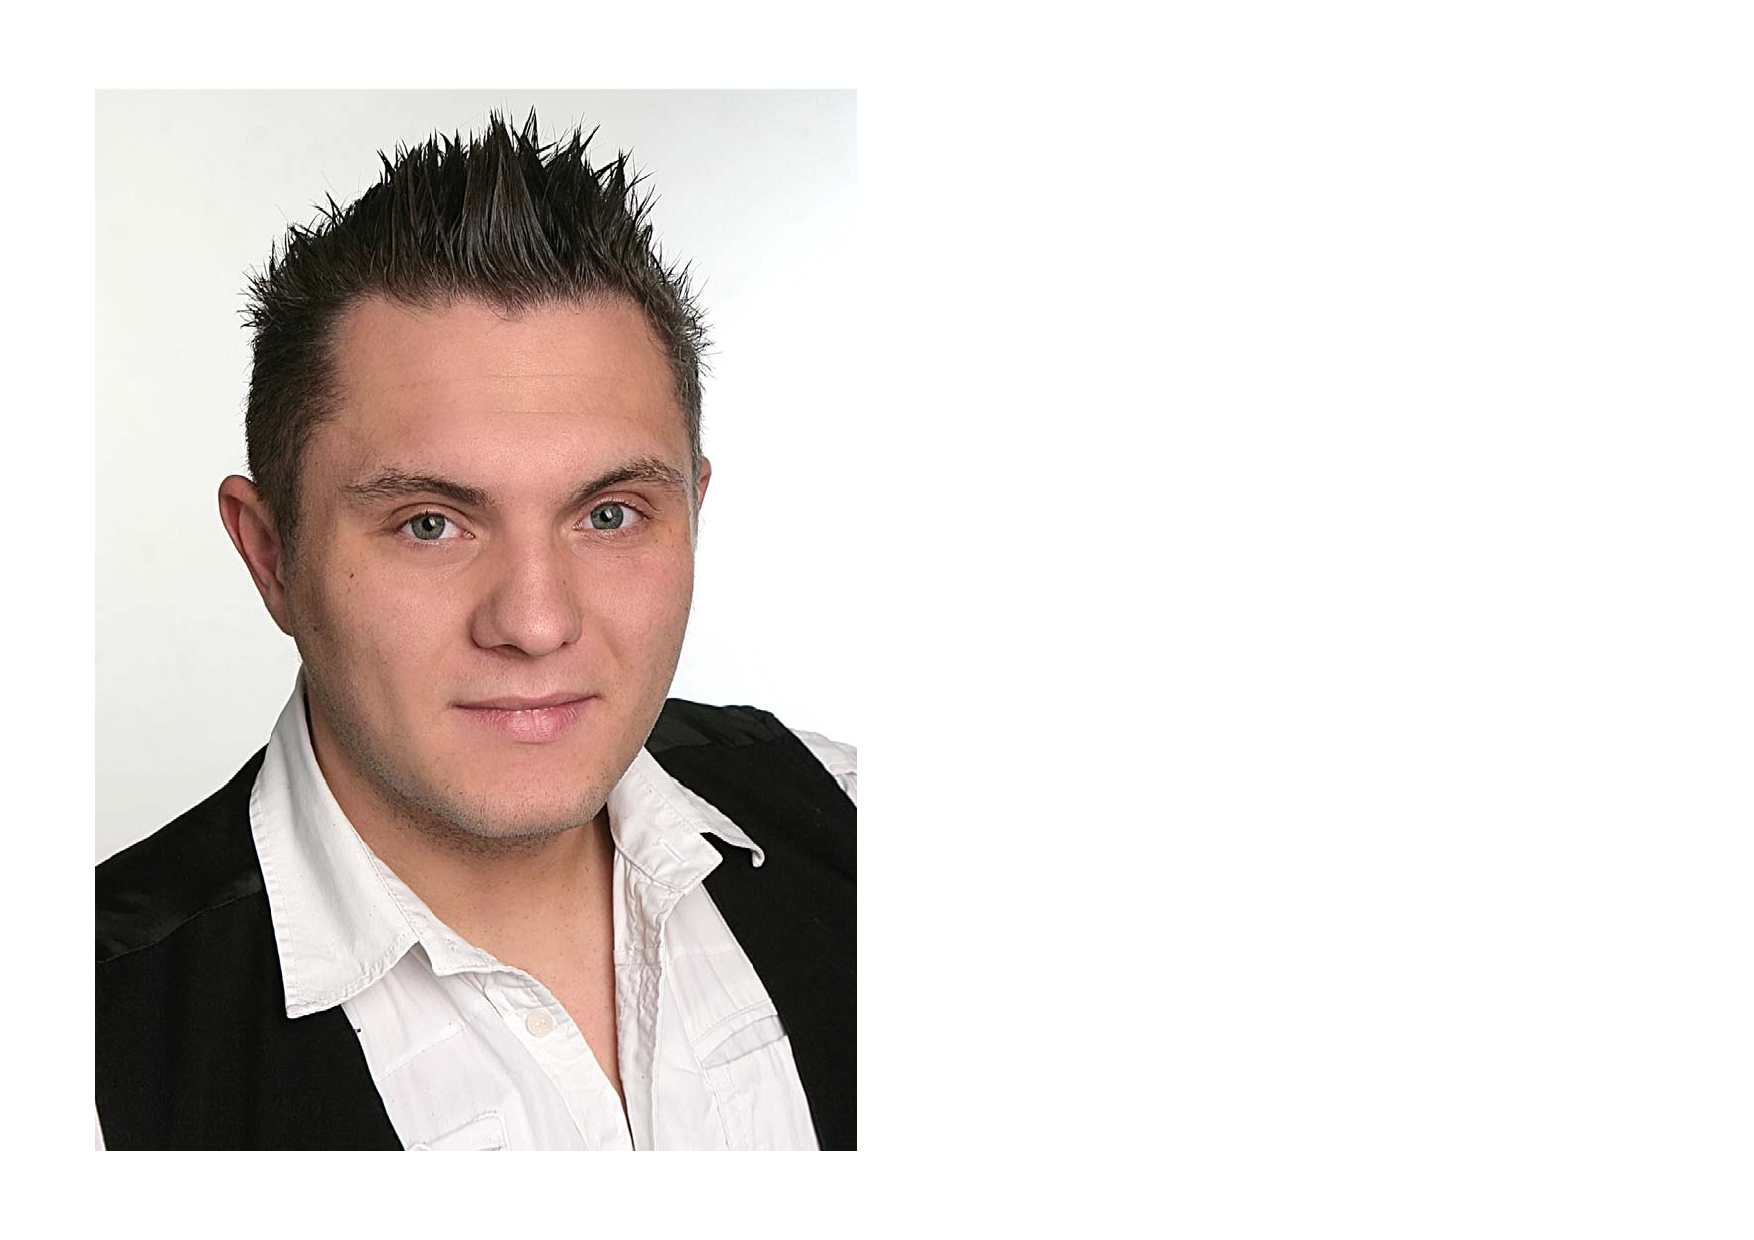
\includegraphics[width=1in,height=1.25in,clip,keepaspectratio]{BT.pdf}}]{Benjamin Ternes}\blindtext \end{biography}%
% or if you just want to reserve a space for a photo:

\begin{IEEEbiography}[{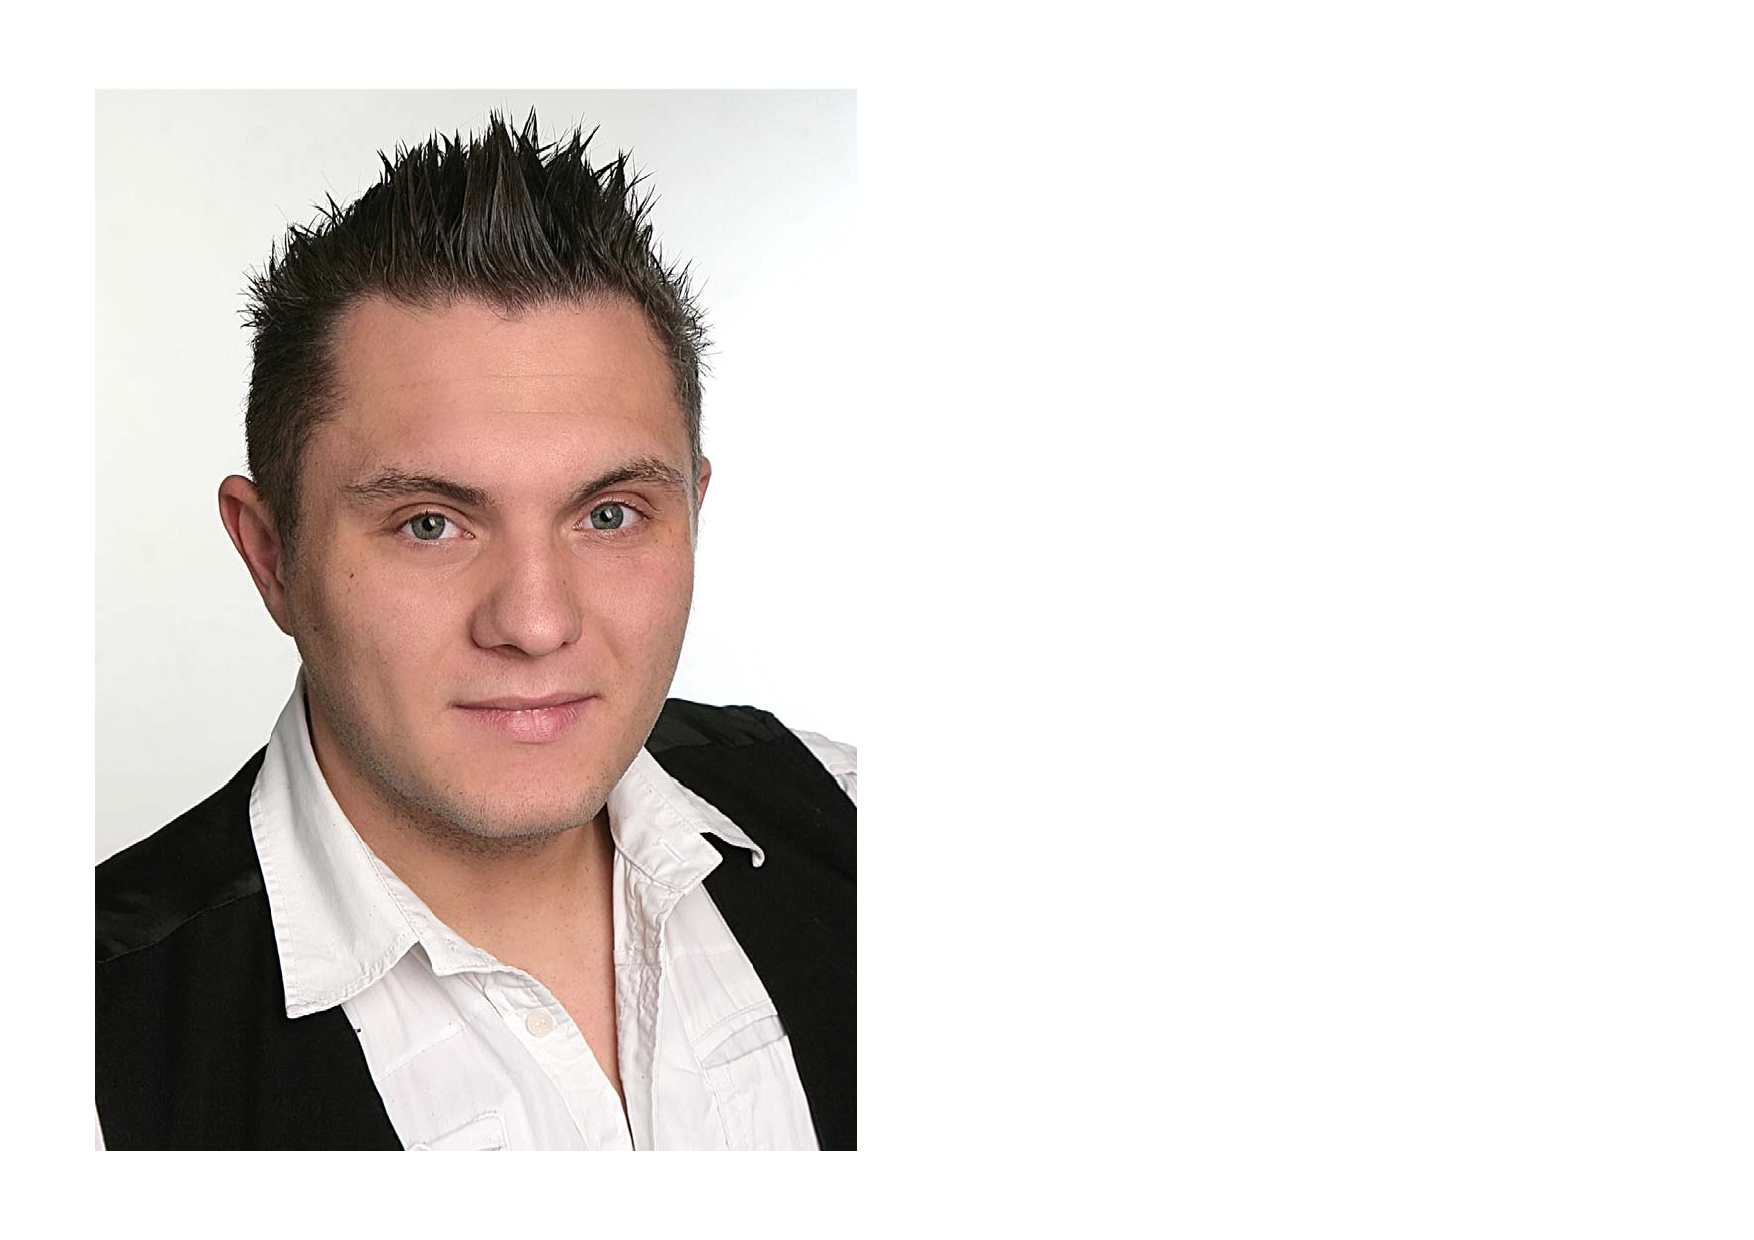
\includegraphics[width=1in,height=1.25in,clip,keepaspectratio]{BT.pdf}}]{Benjamin Ternes}
studierte Elektrotechnik mit dem Schwerpunkt: Antriebs- und Automatisierungstechnik an der FH Dortmund, wo Herr Ternes auch den Abschluss Bachelor of Engineering erlangte. Derzeit ist Herr Ternes an der Hochschule Bochum als Master of Science (Elektrotechnik) eingeschrieben. Seine Forschungsschwerpunkte sind elektrische Maschinen, Systemtheorie und Identifikationsverfahren zur Bestimmung von Maschinenparametern. Nebenbei arbeitet Herr Ternes an der FernUniversität in Hagen als WHF.
\end{IEEEbiography}
% You can push biographies down or up by placing
% a \vfill before or after them. The appropriate
% use of \vfill depends on what kind of text is
% on the last page and whether or not the columns
% are being equalized.

%\vfill

% Can be used to pull up biographies so that the bottom of the last one
% is flush with the other column.
%\enlargethispage{-5in}




% that's all folks
\end{document}


